
\documentclass[calculator,steamtables,refrigeranttables,psychrometricchart,datasheet,solutions,resit]{exam} 
%\documentclass[calculator,steamtables,refrigeranttables,psychrometricchart,datasheet]{exam}

% The full list of class options are
% calculator : Allows approved calculator use.
% datasheet : Adds a note that data sheet are attached to the exam.
% handbook : Allows the use of the engineering handbook.
% resit : Adds the resit markings to the paper.
% sample : Adds conspicuous SAMPLE markings to the paper
% solutions : Uses the contents of \solution commands (and \solmarks) to generate a solution file

\usepackage{pdfpages}
\usepackage{lscape,comment}

\coursecode{EG3521}%%
\coursetitle{Engineering Thermodynamics}%

\examtime{00.00--00.00}%
\examdate{00}{05}{2015}%
\examformat{Candidates must attempt \textit{all} questions.}

\newcommand{\frc}{\displaystyle\frac}
\newcommand{\br}[1]{\!\left( #1 \right)}
\newcommand{\abs}[1]{\left| #1 \right|}
\newcommand{\fracd}[2]{\frac{\mathrm{d} #1}{\mathrm{d} #2}}
\newcommand{\fracp}[2]{\frac{\partial #1}{\partial #2}}
\renewcommand{\d}[1]{\mathrm{d} #1 }
\newcommand{\Ma}{\mathrm{M\!a}}



\begin{document}

\begin{question}

Refrigerant R-22 is used in a geothermal heat pump system (Fig.~\ref{Exam01_Prob4}) in an industrial facility. The heat pump uses underground water from a well to produce a heating capacity of 15 tons. Determine:
\begin{figure}[!h]
\begin{center}
\includegraphics[width=12.0cm,height=9.0cm]{./Pics/Exam_Refrigeration14-15}
\end{center}
\vspace{-1.8cm}
\caption{Heat pump cycle.}\label{Exam01_Prob4}
\end{figure}
\begin{enumerate}[(a)]
 \item Enthalpies and Entropies: h$_{i}$, s$_{i}$ with $i=\left\{1,2,3,4\right\}$;~\marks{8}
\solution{Calculating all properties:
\begin{description}
\item[1:] At P$_{1}$ =  3 bar and T$_{1}$= 21.5$^{\circ}$C $\rightarrow$  T$_{1}$ $>$ T$_{sat}$ (=-14.66$^{\circ}$C), thus the fluid is superheated vapour with \\
${\bf h_{1} = 268.88\text{ kJ.kg}^{-1}}$~\solmarks{1/8} and \\
${\bf s_{1} = 1.03915\text{ kJ.(kg.K)}^{-1}}$.~\solmarks{1/8}
\item[2:] The fluid undertakes an isentropic compression to P$_{2}$ = 24 bar, with \\
${\bf s_{2}=s_{1}}$ {\bf =1.03915  kJ.(kg.K)$^{-1}$}.~\solmarks{1/8} 
$s_{2} > s_{g}\left(P_{2}=24\text{ bar}\right)$, therefore the fluid is superheated vapour with $T_{2} = 131.41^{\circ}C$ and \\
${\bf h_{2} = 332.50\text{ kJ.kg}^{-1}}$.~\solmarks{1/8}
\item[3:] P$_{3}$ = 24 bar and T$_{3}$=T$_{sat}\left(P_{3}\right)$=59.46$^{\circ}$C, with \\
${\bf h_{3} = 121.56\text{ kJ.kg}^{-1}}$~\solmarks{1/8} and \\
${\bf s_{3} = 0.4241\text{ kJ.(kg.K)}^{-1}}$.~\solmarks{1/8}
\item[4:] Isenthalpic expansion to P$_{4}$=P$_{1}$ = 3 bar and \\
${\bf h_{4} = 121.56 \text{ kJ.kg}^{-1}}$~\solmarks{1/8} and \\
In order to calculate the entropy, we need first to calculate the quality of the vapour:
\begin{displaymath}
x_{4} = \frc{h_{4}-h_{f}}{h_{g}-h_{f}} = 0.4321
\end{displaymath}
and~\solmarks{1/8}
\begin{displaymath}
x_{4} = \frc{s_{4}-s_{f}}{s_{g}-s_{f}} = 0.4321 \Longrightarrow {\bf s_{4}=0.4755\text{ kJ.(kg.K)}^{-1}}.
\end{displaymath}
\end{description}
}
%

\item Mass flow rate of the R-22 refrigerant fluid;~\marks{3}
\solution{Energy balance across the condenser with $Q_{H}$ = 15 tons = 52.5 kJ.s$^{-1}$:~\solmarks{3/3}
\begin{displaymath}
Q_{H} = \dot{m}_{R}\left(h_{3}-h_{2}\right)\;\; \Longrightarrow \;\; {\bf \dot{m}_{R} = 0.2499 \text{ kg.s}^{-1}}
\end{displaymath}
}
%

\item Compressor power $\left(W_{C}\right)$ and heat supplied by the evaporator (in kW);~\marks{4}
\solution{Energy balance across the compressor:~\solmarks{2/4}
\begin{displaymath}
{\bf W_{C} =} \dot{m}_{R}\left(h_{2}-h_{1}\right) = {\bf 15.84 kW}.
\end{displaymath}
Energy balance across the evaporator:~\solmarks{2/4}
\begin{displaymath}
{\bf Q_{C} =} \dot{m}_{R}\left(h_{1}-h_{4}\right) = {\bf 36.67 kW}.
\end{displaymath}
}
%
\item Sketch the $Ts$ and $Ph$ diagrams of the cycle indicating all stages, isotherms and isobars.~\marks{5}
\solution{$Ts$ diagram:~\solmarks{2.5/5}
\begin{center}
\includegraphics[width=8.0cm,height=8.0cm]{./Pics/Exam_TS_Refrig} 
\end{center}
$Ph$ diagram:~\solmarks{2.5/5}
\begin{center} 
\includegraphics[width=8.0cm,height=8.0cm]{./Pics/Exam_PH_Refrig}
\end{center}


}
%%


\end{enumerate}
\end{question}



\paperend

%\begin{comment}
%\begin{landscape}
%\begin{center}
%\includegraphics[width=1.5\textwidth]{PsychrometricChart}
%\end{center}
%{
%  \includepdf[pages=-,fitpaper]{./Pics/PsychrometricChart}
%  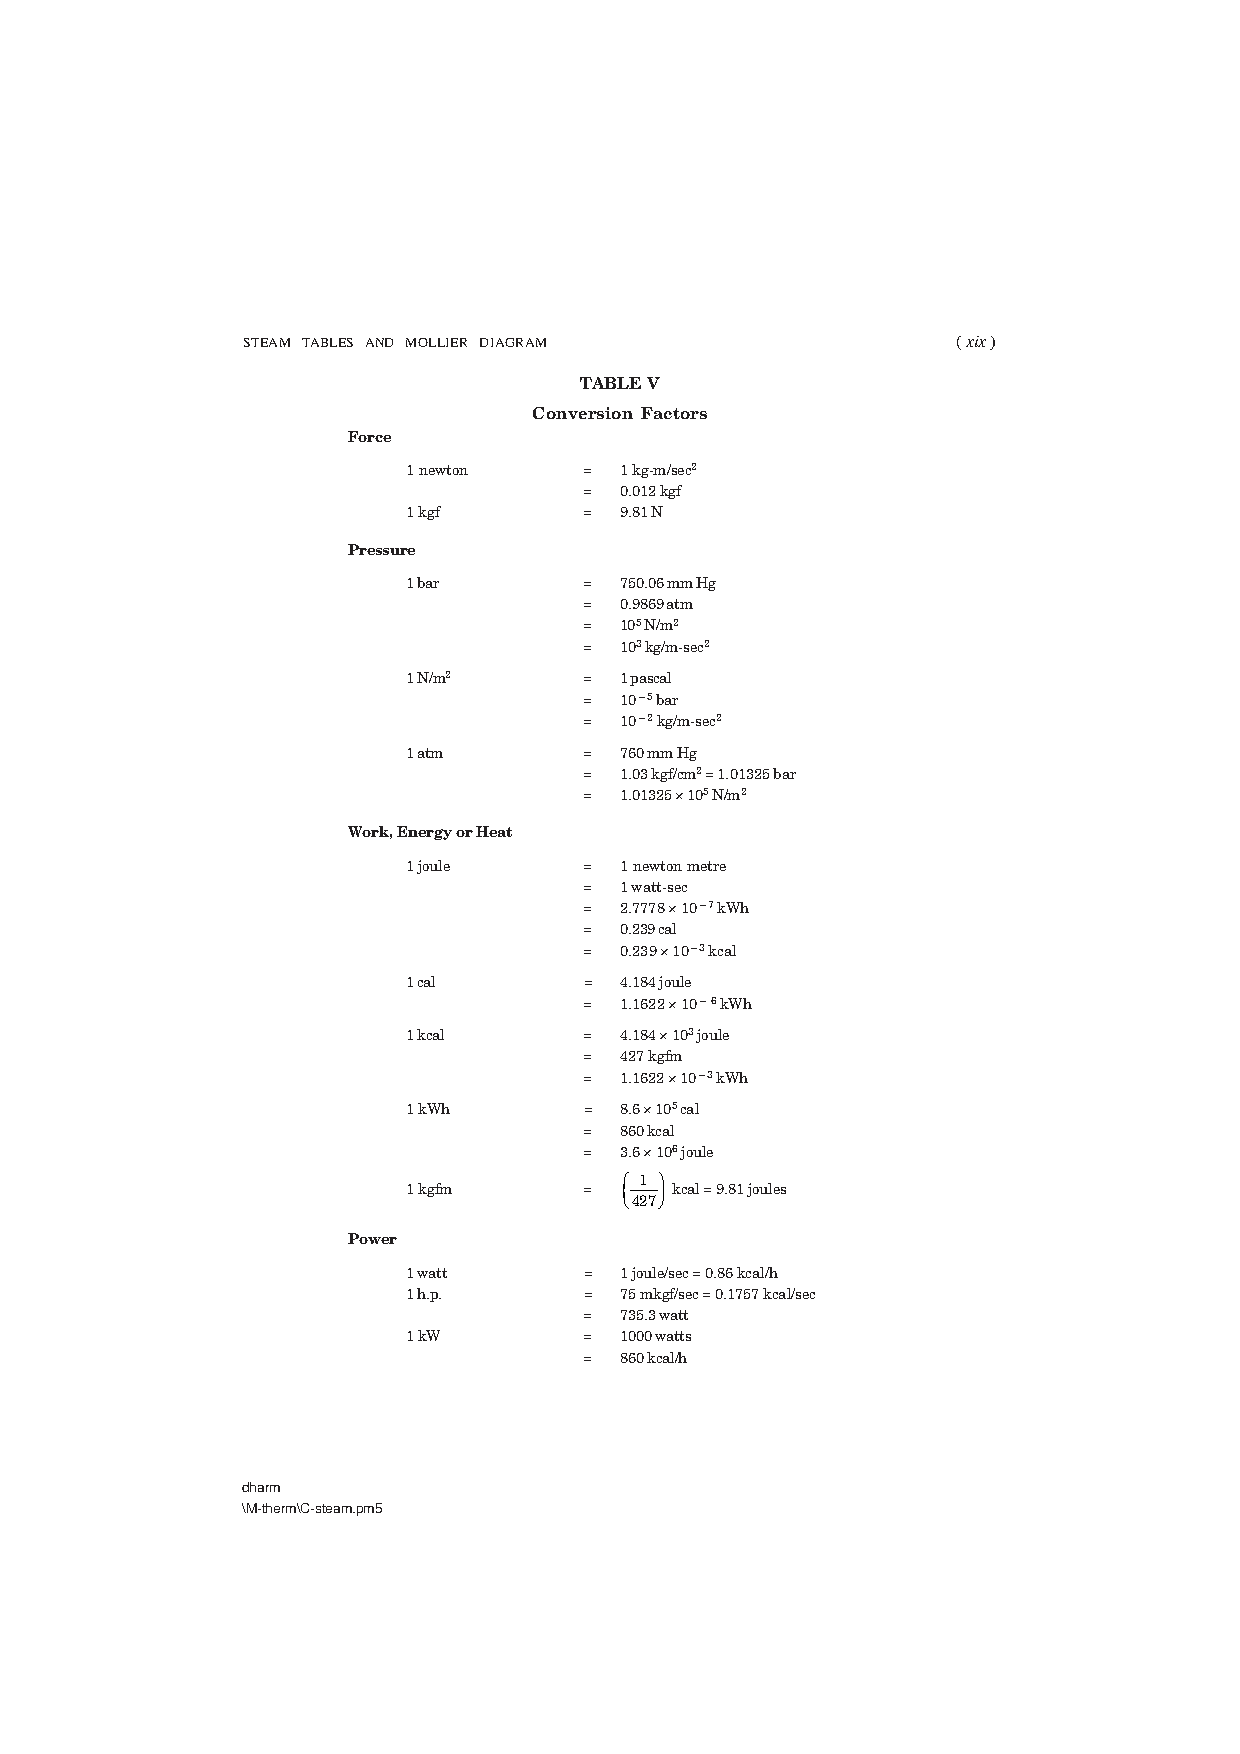
\includepdf[pages=-,fitpaper]{./Pics/UnitsConversion}
%  \includepdf[pages=-,fitpaper]{./Pics/SteamTable_2}
%  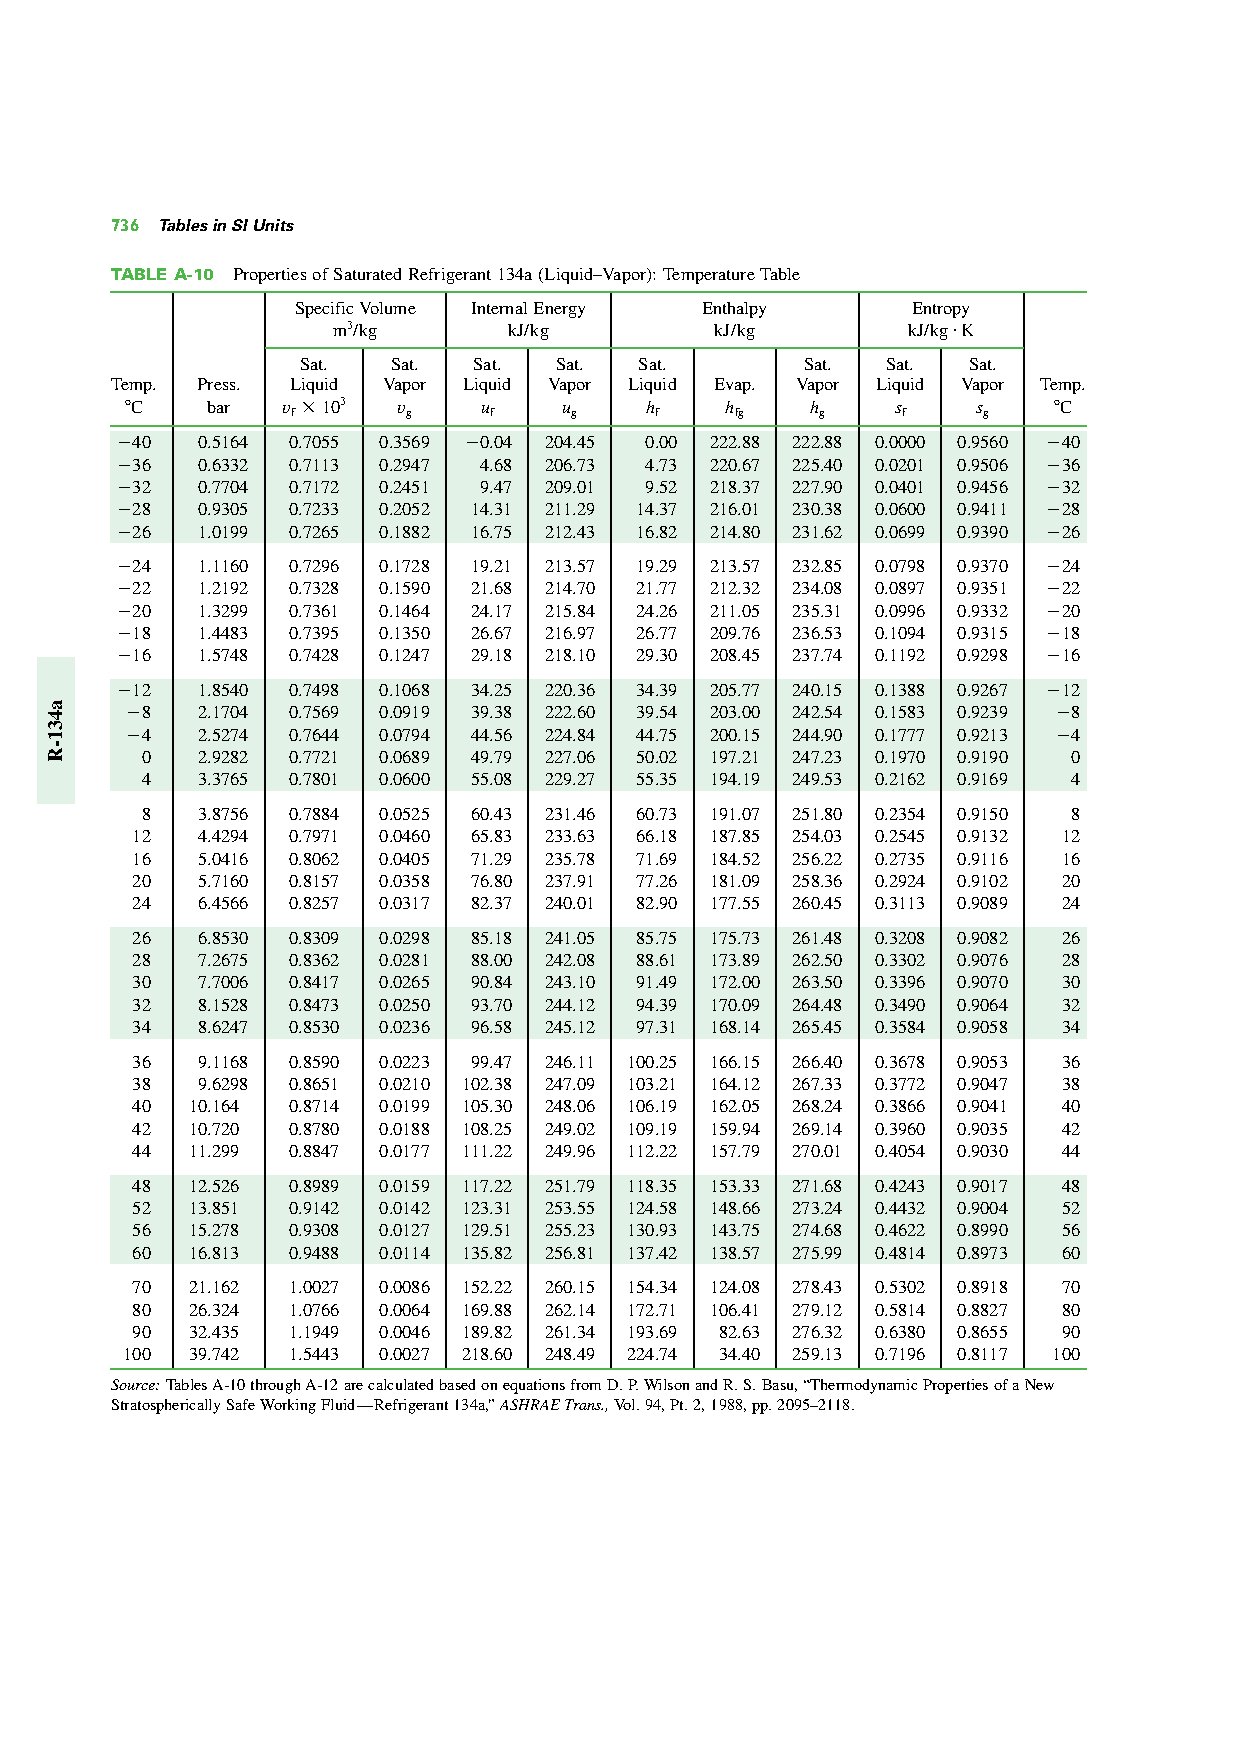
\includepdf[pages=-,fitpaper]{./Pics/Tables_R134}
%}
%\end{landscape}
%\end{comment}

\end{document}
